\documentclass[10pt]{article}
% \usepackage[margin=1in]{geometry}
% \newcommand\hmmax{0}
% \newcommand\bmmax{0}

% % % Fonts% %
\usepackage[T1]{fontenc}
   % \usepackage{textcomp}
   % \usepackage{newtxtext}
   % \renewcommand\rmdefault{Pym} %\usepackage{mathptmx} %\usepackage{times}
\usepackage[complete, subscriptcorrection, slantedGreek, mtpfrak, mtpbb, mtpcal]{mtpro2}
   \usepackage{bm}% Access to bold math symbols
   % \usepackage[onlytext]{MinionPro}
   \usepackage[no-math]{fontspec}
   \defaultfontfeatures{Ligatures=TeX,Numbers={Proportional}}
   \newfontfeature{Microtype}{protrusion=default;expansion=default;}
   \setmainfont[Ligatures=TeX]{Minion 3}
   \setsansfont[Microtype,Scale=MatchLowercase,Ligatures=TeX,BoldFont={* Semibold}]{Myriad Pro}
   \setmonofont[Scale=0.8]{Atlas Typewriter}
   % \usepackage{selnolig}% For suppressing certain typographic ligatures automatically
   \usepackage{microtype}
% % % % % % %
\usepackage{amsthm}         % (in part) For the defined environments
\usepackage{mathtools}      % Improves  on amsmaths/mtpro2
\usepackage{amsthm}         % (in part) For the defined environments
\usepackage{mathtools}      % Improves on amsmaths/mtpro2

% % % The bibliography % % %
\usepackage[backend=biber,
  style=authoryear-comp,
  bibstyle=authoryear,
  citestyle=authoryear-comp,
  uniquename=false,%allinit,
  % giveninits=true,
  backref=false,
  hyperref=true,
  url=false,
  isbn=false,
  ]{biblatex}
\DeclareFieldFormat{postnote}{#1}
\DeclareFieldFormat{multipostnote}{#1}
% \setlength\bibitemsep{1.5\itemsep}
\newcommand{\noopsort}[1]{}
\addbibresource{Thesis.bib}

% % % % % % % % % % % % % % %

\usepackage[inline]{enumitem}
\setlist[itemize]{noitemsep}
\setlist[description]{style=unboxed,leftmargin=\parindent,labelindent=\parindent,font=\normalfont\space}
\setlist[enumerate]{noitemsep}

% % % Misc packages % % %
\usepackage{setspace}
% \usepackage{refcheck} % Can be used for checking references
% \usepackage{lineno}   % For line numbers
% \usepackage{hyphenat} % For \hyp{} hyphenation command, and general hyphenation stuff
\usepackage{subcaption}
% % % % % % % % % % % % %

% % % Red Math % % %
\usepackage[usenames, dvipsnames]{xcolor}
% \usepackage{everysel}
% \EverySelectfont{\color{black}}
% \everymath{\color{red}}
% \everydisplay{\color{black}}
% % % % % % % % % %

\usepackage{pifont}
\newcommand{\hand}{\ding{43}}
\usepackage{array}


\usepackage{multirow}
\usepackage{adjustbox}

\usepackage{titlesec}

\makeatletter
\newcommand{\clabel}[2]{%
   \protected@write \@auxout {}{\string \newlabel {#1}{{#2}{\thepage}{#2}{#1}{}} }%
   \hypertarget{#1}{#2}
}
\makeatother

% \newcommand{\boxarrow}{%
%   \mathrel{\mathop\Box}\mathrel{\mkern-2.5mu}\rightarrow
% }
% \newcommand{\diamondarrow}{%
%   \mathrel{\mathop\Diamond}\mathrel{\mkern-2.8mu}\rightarrow
% }

\usepackage{multicol}

\setcounter{secnumdepth}{4}
\setcounter{tocdepth}{4}

\usepackage{tikz}
\usetikzlibrary{arrows,positioning}

\usepackage{tabularx}

\usepackage{bussalt}
\usepackage{Oblique} % Custom package for oblique commands
\usepackage{CustomTheorems}

\usepackage[hidelinks,breaklinks]{hyperref}

\title{Oblique Reasoning}
\author{Ben Sparkes}
% \date{ }

\begin{document}
\maketitle

Central idea is that the evaluation of options is not necessarily made on the basis of information available to an agent.

We're familiar with the idea that there may be a distinction between an agent's `true' evaluation and some ersatz evaluation that guides their practical reasoning (perhaps worth noting that ersatz can be seen as arising from failures of transparency).
For example, in cases of akrasia, weakness of will, and so on.
However, the argument here is that there doesn't even need to be a ersatz evaluation for an agent to engage in practical reasoning.
Parts of an agent's evaluation may be inaccessible but still guide an agent's reasoning.
{\color{red} (This I think is new, or fairly under-explored. The standard understanding of practical reasoning is a special case, and the more general case is kind of interesting.)}

On the logic side, develop a formalism to capture the background structure.
This doesn't account for the specific reasoning, but it does something to set up a framework for explaining the basic principles and suggesting how the basic idea can be extend to decision theoretic contexts, etc.


This doesn't directly reduce to a kind of cognitivism, though it comes close.
Roughly, if cognitivism holds, then the central thing is belief about what's `good', and one can view this all in terms of a cognitivist structure, in which one's means are providing evidence of a kind, but I don't think it follows that this is the way to do the work.
Rather, it's a familiar gloss.
But, you need more to get the cognitivist picture going\dots
Unless, of course, the picture is that cognitivist just amounts to there being reasoning involved, and hence in contrast to a kind of struct Humean position.

Perhaps useful to contrast Broome's ``core type'' of reasoning in `Rationality through reasoning', as this involves language of a kind, etc.

Reflection principles!


\section{Notes on the interpretation}
\label{sec:notes-interpretation}

Here, the basic idea is that there's some kind of evaluative function that's specifying beliefs and desires, and the modal is picking up something of a threshold.
This can be seen as binary, etc.\ but the important thing is that there's nothing to special about the set of situations.
Either these are those for which the valuation is `true', or there's some relevant threshold, etc.\ but more generally the same evaluative principle can be applied to other states, and with this I can reason about means, ends, and the like from the perspective of desires, beliefs, and more.
It's in this sense that these are propositional attitudes.
Again, this goes back to the idea of tests, which I don't think fits into the broad picture that I'm trying to motivate here, but \dots

This probably contrasts to the \(O\phi \coloneq G \rightarrow \phi\) approach, as here there's an explicit proposition that's the good, and it's the logical relation this has to other states which is important.
So, no propositional attitude, at least on a fairly natural interpretation.


\section{Notes on the formalism}
\label{sec:notes-formalism}

Given the way I've set things up, I think I have \(\attn{\lnot\phi} = \lnot\attn{\phi}\).
In particular, this should probably follow from the fact about how transplication and negation interact.
Though, this isn't currently stated as a fact.

Failure of cloaure under negation for the oblique fragment, and closing under negation as the way to figure out the recognised situations.
However, this means that I don't have an \emph{abstract modal logic} in the blue books sense of the term (p.\  476).
But temporal logic ain't an abstract modal logic, so this failure isn't too interesting.

`The best introduction to expressive completeness is the encyclopedic Gabbay, Hodkinson, and Reynolds [163]; both separability and game-based proofs are discussed. It also contains many other results on since and until logic and a useful bibliography.'

Possibly easier to axiomatise what's going on by using a kind of global modality.
This is inspired by \citeauthor{van-Benthem:1979aa}'s ideas about Leibniz's ideas of permissibility and so on.
However, on \citeauthor{van-Benthem:1979aa}'s approach, there's a modality picking up on the accessible worlds, whereas with what I'm interested in, I want the accessibility relation to be genuinely global.
This, is likely a problem.
Oh, following the blue book, the global modality alone has a decidable satisfiability problem.
The axiomatisation is seemingly simple too, with the standard S5 axioms being supplemented with \emph{inclusion}:
\[\Diamond p \rightarrow E\phi\]
Where \(Ep\) means that there's some \(p\) world in the model.
And, this apparently applies to normal modal logics quite generally.
Interesting that this global modality can't define irreflexivity.
If permissibility is able to do this, then there are probably questions about decidability.

From Gargov, Passy, Tinchev, it looks as though standard canonical model type constructions can be used to prove completeness for the box and window logic.
And, I have a feeling this should also work for partial logic.
A difficulty might be in generating MCSs, but here maybe either treat negations properly, or introduce an additional syntactic component to identify lack of truth value.
I mean, in a sense these aren't going to be MCSs, as adding some atomic expression would likely preserve consistency, while also violating the idea that arbitrary atomic expressions can be undefined.

\begin{enumerate}
\item \(\attn{\phi} \rightarrow \phi\), to ensure appropriate subset relation.
\end{enumerate}

I think this is the only thing required.
And, the reason to be interested in MCSs is to ensure one considers every `possible world'.
This is useful for finding counterexamples.
An additional syntactic component to capture undefinedness should be fine.
The partial operator(s) may be a little more difficult, but this isn't obvious.



\newpage

A stack of articles is at rest on my desk.
The yellow post-it note stating ``for research idea'' indicates that the stack was put to rest.
Some time ago I fixed some end, some research idea, and the articles were assembled as means to that end.
Some thing interrupted my performance of the means, and I can not now recall the idea to which the articles were a means to pursuing.
However, the organisation of the stack and light annotation to some pages suggest I may be able to recall the research idea by working through the stack.

My reasoning about whether to read the articles is an instance of mundane scenarios in which the instrumentalist means-end structure of practical reasoning is inverted.
In these scenarios, an agent recognises means to some end, but does not have the resources to reason about the end.
And, in turn, the agent recognises that their present evaluation of the means may diverge from their evaluation of the means were they to have to the resources to reason about the end.
Without the ability to reason about the research idea, I lack the ability to appropriately evaluate working through the stack.
For, were I able to reason about the research idea that the stack of papers were a means to, I would be able to evaluate the idea and in turn of whether to work through the stack.
If were to no longer view the idea as viable it may be that I should pursue some other activity, while if I still regard the idea as viable I have an activity set out for me.

Let us term this end-means reasoning.
End-means reasoning is not the strict inverse of standard means-end reasoning.
For, means-end reasoning typically proceeds from some recognised end to recognised means, while end-means reasoning requires some representational lacuna.
The stack of articles were a means to finding something sensible to say about cases of end-means reasoning, working through the stack was valuable given this end, and I reasoned that this end was worthwhile pursuing despite my inability to reason about it directly.
And, we are here because I was successful in reconstructing the end after pursuing the means to it.

What I have to say about end-means reasoning is fairly straightforward.
We are agents with bounded resources, and some of these bounds relate to the possibilities we are able to reason about.
Cases of end-means reasoning arise when changes in our representational resources lead to the inability to recognise possibilities that was previously identified as an end, though the resources required to represent chosen means toward that end persist.
This lack of representational resources then indicates to the agent that the evaluative judgements they can make may diverge from those they would make given additional representational resources, but their recognition of the specified means as means allows them to indirectly reason about the evaluative judgements they may make given additional representational resources.\nolinebreak
\footnote{TODO: Simplify this! The key point is that the agent's practical reasoning isn't premised on their current evaluative judgements.
  In this respect, the issue is very similar to the way I've been thinking about cases of temptation.
  An agent attempts to reason about what their `more refined' evaluative judgements would be.
  This is also super close to what Smith does with ideal advisers, but without the ideal part (and I think for a fairly different application).
}

In this respect, end-means reasoning is an instance of \emph{oblique} reasoning; reasoning which goes beyond the representational resources that you have at your disposal.
\begin{center}
  [More to say here\dots]
\end{center}

The goal is to make this sketch into a precise analysis.
In doing so I hope to show that cases of end-means reasoning can complement whatever your understanding of practical reasoning is.
In turn, I hope that your understanding of practical reasoning helps shed light on normative and descriptive aspects of end-means reasoning.
This assumes that your understanding of practical reasoning does not rule out the possibility of end-means reasoning, but beyond this the specific account of end-means reasoning I give is meant to be illustrative.
The analysis is framed in terms of more-or-less well explored formal treatments of folk theory.
I will explain and augment this framework as required, but I expect you to translate the analysis to any other framework as you see fit.


Aim to show some degree of continuity!


\begin{center}
  [\textbf{Structure of the paper.}]
\end{center}

\newpage

The important idea with these types of cases isn't the way reasoning is structured, but how ends function, I think.
In that, with the record store case, the supermarket case, and so on, the broad instrumentalist picture of practical reasoning can be preserved.
The end is still fixed, and so you can have the `end' of completing the means, but this won't have much actionable content.
The thing is that this isn't really a new end, rather this is a redescription of the same end, and something like this is always going to be possible with the kind of cases I've set up.
Hence, the claim that the reasoning is different is due to the relative importance of the means, etc.
In standard cases, you can always reevaluate the means with respect to the end that they're a means to, whereas here, there's no way to figure out whether they should be developed/reformed etc.

What's important, is that there's no straightforward way to evaluate the actions compatible with your means.
In this respect, the relevant reasoning can't be weighing up reasons for an against, etc.\ because there's no way to recognise those reasons, speaking loosely.
Similarly, perceived desirability and so on seem problematic.
From a different point of view, there's some full evaluation function, and the agent only has restricted access to it.

So, an idea is that this is a special case of weakness/strength of the will.
For, in these cases the desirability of the means may drop below the desirability of other courses of action.
However, you see that there's something missing in your evaluation, and you may still pursue the means.

In terms of reasons, there's the contrast between considering all of the reasons for and against an action, and considering those which are `available' to you.
And, in the cases I'm thinking of, you're not interested in all the reasons for and against, but you're still interested in reasons which go beyond what are available to you.

In part, this is because the reasons that are no longer available to you did impact your evaluation of actions, and you still have some information about this.

So, the general perspective on practical reasoning that I want to pursue here is one in which evaluative judgements are foundational but do not exhaust practical reasoning.
And, approaching this from the perspective of propositional attitudes gives something very coarse grained.
It allows one to kind of see how the partiality is functioning, but if the relevant judgements rely on any kind of comparative notion, then the model won't have the resources to capture this.
Exploring the more fine grained comparisons doesn't look too straightforward, either.
One way of doing this, though, would be to assume that there's an evaluative function on situations.
For if this is the case, then the evaluation of complex expressions can be treated compositionally, and hence a more fine grained evaluation can be tied to a partial denotation.

With these examples, what needs to be stressed is that you're not relying on your current evaluative judgement regarding the means that you have selected.
Rather, you're relying on some other evaluative judgement.
Hence, there's some kind of end-means reasoning, in terms of how one's evaluative judgements are being formed.
Usually, the evaluation of means proceeds from the evaluation of ends, but here it's almost the other way round.

% Due to the means-end structure of the relevant reasoning here, it's not clear that this straightforwardly hooks up to issues about incomplete preferences.
% For, on my understanding, this primarily concerns how to make evaluative judgements, whereas here it seems as though no explicit evaluative judgement is required, or going to be of any substantial help, as the appropriate evaluation of the options available to you is there, but inaccessible.

% The way I'm thinking about means and ends seems to be close to how \citeauthor{Bratman:1987aa} thinks about intentions.
% Roughly, the specification of an end narrows down one's desires, but this isn't given by one's desires, etc.\ so it can't simply be a mental state on par with desire.



\newpage

\section{Formalism}
\label{sec:formalism}

Two things we need to capture.
Our theoretical perspective and the agent's perspective.

Standard treatment of propositional attitudes.
Collections of situations.

\begin{definition}[Frame]
  A \emph{frame} \(\oframe{F}\) is a pair \((S,\langle A_{1},\dots,A_{n} \rangle)\) where
  \begin{itemize}
  \item \(S\) is a collection of points capturing situations,
  \item Each \(\fatt{} \colon S \to \wp(S)\) is a function associating to each situation a subset of situations which are compatible with the agent's attitde.
  \end{itemize}
  Attitudes may satisfy certain requirements, e.g.\ if \(t \in \fatt{u}\) then \(\fatt{t} = \fatt{u}\), etc.
\end{definition}
A frame can be augmented to include further distinguished subsets, and multiple distinguished subsets corresponding to multiple agents may be intruded.
Frames fix the situations and what the agent `desires' and `believes' independently of the resources we have to reason about these.
{\color{red} This should be reformulated.
  What's required here are `desire-like' and `belief-like' attitudes.
  The former can the correspond to desires, ends, and the like, while the latter to beliefs, means, and the like.
  And, frames should permit (at least) finite collections of these.}

\emph{Expressions} builts from some langauge are used to talk about a frame, and our primary interest will be in the \emph{propositions}, or collections of situations, that expressions refer to.
Key to our understanding of oblique attitudes is capturing the appropriate expressive power of a language with respect a frame, but nothing rests on our use of the terms `proposition' and `expression' other than this distinction between aspects of a language and their interpretation.

\begin{definition}[Propositions]
  Subsets of the collection of situations.
  Specified with respect to a frame.
\end{definition}

\begin{definition}[Atomic Expressions]
  Set of symbols \(\mathsf{Exp}\), non-logical.
\end{definition}

Every expression denotes a proposition, but it does not follow that for every proposition there is a corresponding atomic expression.
Resources are captured via interpreting the frame through expressions which denote collections of situations.
Hence, agents aren't necessarily able to reason about arbitrary collections of sitations.
Instead, the agent has expressions, and their reasoning is bounded by the collections of situations that these refer to.
And, there's no guarantee that any given collection of sitatuations is characterised by an expression.
While we have only introduced atomic expressions, this claim extends to arbitrary expressions, detailed below.

Propositional attitutdes are understood with respect to this characterisation of propositions.
Hence, for an agent to have an attitude toward a proposition is not for an agent to have an attitude toward an expression.
Rather, for an agent to have an attitude toward a proposition is for there to be a relation between an agent and a collection of sitautions.
In turn, this is a coarse grained perspective on the functional profile of an agent.
For example, the \emph{beliefs} of an agent are captured through the proposition corresponding to the situations they are unable to distinguish from the actual situations.
The \emph{desires} of an agent are captured by collecting the situations in which they would be satisfied.
Likewise, the \emph{means} and \emph{ends} adopted by an agent may be characterised through compatible situations.



Rare that an agent will identify a unique sitaution.
Indeed, if an agent can uniquely identify each sitaution, then they may be able to reason about arbitrary propositions.
In part this captures bounded resources.
Though, this aspect of bounded agency is captured quite generally, whether it is made explicit or not.\nolinebreak
\footnote{Indeed, it follows from some natural formal constraints.
  For, given an infinite set of situations, there are uncountably many collections of situations, and languages are typically restricted to countably many expressions.}
Primary sense of a resource is being able to put a proposition to some use.
Expressions, then, amount to resources, as do the attitudes specified at the frame level.

To capture reasoning regarding oblique attitudes we separate two distinct ways a given atomic expression can be put to use by an agent.

First, there is the \emph{support} that an expression gives to an agent's reasoning.
The support of an expression identifies those situations which are compatible with the expression and those which are incompatible with the expression.\nolinebreak
\footnote{We use the terms `compatible' and `incompatible' as generic placeholders.
  For, while we assume that the support of an expression amounts to the truth conditions of an expression, this is merely a simplifying assumption.
  Gaps and gluts may inform the backdrop of an agent's reasoning, but these are potential complications that we set aside at present.}
Second, there is the \emph{application} of an expression in an agent's reasoning.
These are the situations that an agent takes to be compatible and incompatible with the expression.

Key to our analysis is the idea that an agent's reasoning may only apply to a subset of the situations supported by an expression.
In this respect, an agent's application of an expression may be \emph{partial}.

\begin{center}
  [Explanation of examples]
\end{center}

\begin{figure}[ht]
  \centering
  \begin{subfigure}[b]{0.3\textwidth}
    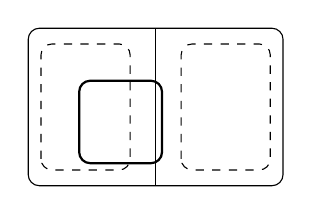
\begin{tikzpicture}
      \pgfmathsetmacro\gr{1.61803}
      \pgfmathsetmacro\by{2}
      \pgfmathsetmacro\bx{\by*\gr}
      \draw[rounded corners] (0,0) rectangle (\bx,\by);

      \draw (\bx/2,0) -- (\bx/2,\by); % Centre division

      \draw[rounded corners, thick] (\bx*0.2, \by/1.5) rectangle (\bx*0.525,\by/7);

      \draw[rounded corners, dashed] (\bx*0.05, \by*0.1) rectangle (\bx*0.4,\by*0.9);
      \draw[rounded corners, dashed] (\bx*0.6, \by*0.1) rectangle (\bx*0.95,\by*0.9);
    \end{tikzpicture}
    \caption{}
  \end{subfigure}
  \begin{subfigure}[b]{0.3\textwidth}
    \centering
    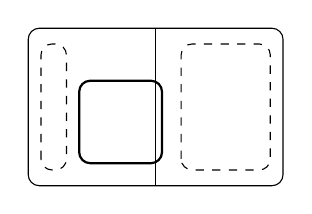
\begin{tikzpicture}
      \pgfmathsetmacro\gr{1.61803}
      \pgfmathsetmacro\by{2}
      \pgfmathsetmacro\bx{\by*\gr}
      \draw[rounded corners] (0,0) rectangle (\bx,\by);

      \draw (\bx/2,0) -- (\bx/2,\by); % Centre division

      \draw[rounded corners, thick] (\bx*0.2, \by/1.5) rectangle (\bx*0.525,\by/7);

      \draw[rounded corners, dashed] (\bx*0.05, \by*0.1) rectangle (\bx*0.15,\by*0.9);
      \draw[rounded corners, dashed] (\bx*0.6, \by*0.1) rectangle (\bx*0.95,\by*0.9);
    \end{tikzpicture}
    \caption{}
  \end{subfigure}
  \begin{subfigure}[b]{0.3\textwidth}
    \centering
    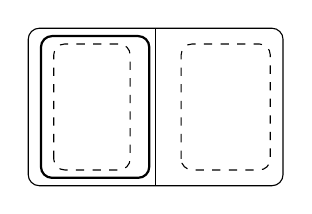
\begin{tikzpicture}
      \pgfmathsetmacro\gr{1.61803}
      \pgfmathsetmacro\by{2}
      \pgfmathsetmacro\bx{\by*\gr}
      \draw[rounded corners] (0,0) rectangle (\bx,\by);

      \draw (\bx/2,0) -- (\bx/2,\by); % Centre division

      \draw[rounded corners, thick] (\bx*0.05, \by*0.05) rectangle (\bx*0.475,\by*0.95);

      \draw[rounded corners, dashed] (\bx*0.1, \by*0.1) rectangle (\bx*0.4,\by*0.9);
      \draw[rounded corners, dashed] (\bx*0.6, \by*0.1) rectangle (\bx*0.95,\by*0.9);
    \end{tikzpicture}
    \caption{}
  \end{subfigure}
  \caption{Application examples}
\end{figure}

From a formal point of view, the support and application of an expression are both instances of what we term a \emph{denotation}; a pair of functions mapping an atomic expression to those compatible and incompatible situations, respectively.

\begin{definition}[Denotation]
  Given a frame \(\oframe{F}\) and set of atomic expressions \(\atmexp\), a \emph{denotation}, \(D = \langle \cdeno{},\ideno{} \rangle\), is a pair of functions
  \begin{align*}
    \cdeno{} \colon \mathsf{Exp} \to \wp(S) & & \ideno{} \colon \mathsf{Exp} \to \wp(S)
  \end{align*}
  such that for every \(P \in \mathsf{Exp}, \cdeno{P} \cap \ideno{P} = \emptyset\).

  If for every \(P \in \mathsf{Exp}\) we have \(\cdeno{P} \cup \ideno{P} = S\), then we call the denotation \emph{full}.\newline
  Else, we call the denotation \emph{partial}.
\end{definition}

Given two denotations \(D_{1} = \langle \cdeno[d_{1}]{},\ideno[d_{1}]{} \rangle\) and \(D_{2} = \langle \cdeno[d_{2}]{},\ideno[d_{2}]{} \rangle\), if for all \(P \in \mathsf{Exp}\),
\begin{enumerate*}[label=]
\item \(\cdeno[d_{1}]{P} \subseteq \cdeno[d_{2}]{P}\) and
\item \(\ideno[d_{1}]{P} \subseteq \ideno[d_{2}]{P}\),
\end{enumerate*}
then we say that \(D_{1}\) is a \emph{restriction} of \(D_{2}\) or, conversely, that \(D_{2}\) is an \emph{expansion} of \(D_{1}\).

Full denotation can be taken to correspond to truth conditions.
This is the intended perspective.
Application is then the way the agent applies these truth conditions.
However, this can be seen as an idealising assumption that one may not want to make.
Allowing an agent to diverge can be useful.





To \emph{interpret} a collection of atomic expressions with respect to some frame, then, we require a pair of related denotations.
First a full denotation to capture to the support of any atomic expression and second a potentially partial denotation to capture its application.

\begin{definition}[Interpretation]
  Given a collection of atomic expression \(\mathsf{Exp}\) and a frame \(\oframe{F}\), an interpretation, \(\mathcal{I} = \langle \mathcal{S},\mathcal{A} \rangle\), is a pair of denotations where \(\mathcal{A}\) may be partial denotation and \(\mathcal{S}\) is a full denotation expanding \(\mathcal{A}\).
\end{definition}

{\color{red} Intuitively, \dots this means that we can treat \(\mathcal{S}\) as providing truth conditions and \(\mathcal{A}\) as providing an agent's application of these truth conditions.}

Given a collection of atomic expressions, a frame paired with an interpretation forms a model.

\begin{definition}[Model]
  An \emph{oblique model} \(\omodel{M} = \langle \oframe{F}, \ointp{I} \rangle\) is a frame together with an interpretation.
\end{definition}

Given a scenario, the specification of a model captures core aspects of the phenomena we are interested in.
For, we can state what beliefs and desires an agent has, we can then study how atomic expressions relate to an agent's beliefs and desires, the relations which hold between atomic expressions, and the result of composing atomic expressions to form complex expressions.
As in the examples above, natural language is adequate for this task.
%TODO Maybe say more here
Still, introducing a formal language affords us an easier investigation of complex models and helps fix the foundation for a systematic study of models in general.

The logical language we use to reason about complex expressions, interplay between the support and application of expressions, and the desires and beliefs of agents is a generalisation of the basic modal language.
We include the standard logical operations of negation and conjunction, two modalities to capture the desires and beliefs of the agent, and two additional \emph{oblique} operators to reason about the application of expressions by an agent.

\begin{definition}[Oblique language]
  Given a collection of atomic expressions \(\mathsf{Exp}\), the well-formed expressions \(\phi\) of an \emph{oblique language} \(\olang{}\) are given by the following rule:
  \[
    \phi \Coloneqq P \in \mathsf{Exp} \bnfsep \lnot\phi \bnfsep \phi\land\psi \bnfsep \phi\lor\psi \bnfsep \lattu[A_{i}]{\phi} \bnfsep \lattd[A_{i}]{\phi} \bnfsep \attn{\phi} \bnfsep \phi \ltrans \psi
  \]
\end{definition}

Given that an interpretation of a frame consists of two denotation functions which are themselves pairs, the way in which we understand expression in given oblique language requires some care.
First, we shall treat expressions as referring to the situations they are compatible with, and use negation of an expression (\(\lnot\)) to refer to those situations incompatible with the expression.
Second, we will default to taking an expression to refer to its support.
The unary operator \(\attn{\cdot}\) is then given to indicate the application of an expression.\nolinebreak
\footnote{Either we must fix our understanding of an expression relative to a denotation, or we must provide a way to switch from one denotation to another.
  Either option is viable, but we chose the latter as this affords us the ability to mix the support and application of an expression when building complex expressions.
This ability is useful to have, as we can the express relations which hold between our perspective and the agents.}

For example, \(P\) is be read as referring to the situations which are compatible with the support of \(P\), while \(\attn{P}\) is read as referring to the situations compatible with the application of \(P\).
Complex expressions may combine both support and application.
Hence, \(P \land \attn{\lnot Q}\) will refer to the situations which are compatible with the support of \(P\) and are incompatible with the application of \(Q\).

The binary operator \(\cdot \ltrans \cdot\) serves as a restrictor of sorts.
The expression \(\phi \ltrans \psi\), reads `\(\phi\) is compatible with all the situations compatible with \(\psi\)'.
\(\attn{\phi} \ltrans \phi\) will always hold, as the application of \(\phi\) always denotes a subset of the support of \(\phi\), however \(\phi \ltrans \attn{\phi}\) may not hold, as an agent may fail to consider some \(\phi\) situations in their application of the expression.

\begin{figure}[ht]
  \centering
  \begin{subfigure}[b]{0.4\textwidth}
    \centering
    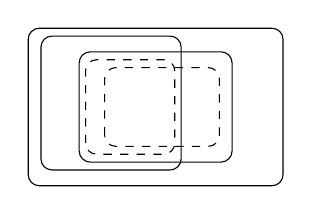
\begin{tikzpicture}
      \pgfmathsetmacro\gr{1.61803}
      \pgfmathsetmacro\by{2}
      \pgfmathsetmacro\bx{\by*\gr}
      \draw[rounded corners] (0,0) rectangle (\bx,\by);

      \draw[rounded corners] (\bx*0.05, \by*0.1) rectangle (\bx*0.6,\by*0.95);

      \draw[rounded corners, dashed] (\bx*0.225,\by*0.2) rectangle (\bx*0.575,\by*0.8);

      \draw[rounded corners] (\bx*0.2, \by*0.15) rectangle (\bx*0.8,\by*0.85);

      \draw[rounded corners, dashed] (\bx*0.3,\by*0.25) rectangle (\bx*0.75,\by*0.75);
    \end{tikzpicture}
    \caption{\(Q \ltrans \attn{P}\), \(\sim(Q \ltrans P)\)}
  \end{subfigure}
  \begin{subfigure}[b]{0.4\textwidth}
    \centering
    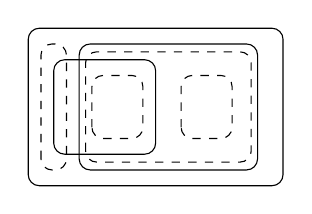
\begin{tikzpicture}
      \pgfmathsetmacro\gr{1.61803}
      \pgfmathsetmacro\by{2}
      \pgfmathsetmacro\bx{\by*\gr}
      \draw[rounded corners] (0,0) rectangle (\bx,\by);

      \draw[rounded corners] (\bx*0.1, \by*0.2) rectangle (\bx*0.5,\by*0.8); % P
      \draw[rounded corners] (\bx*0.2, \by*0.1) rectangle (\bx*0.9,\by*0.9); % Q

      \draw[rounded corners, dashed] (\bx*0.05, \by*0.1) rectangle (\bx*0.15,\by*0.9); % a~Q
      \draw[rounded corners, dashed] (\bx*0.225, \by*0.15) rectangle (\bx*0.875,\by*0.85); % aQ
      \draw[rounded corners, dashed] (\bx*0.6, \by*0.3) rectangle (\bx*0.8,\by*0.7); % a~P
      \draw[rounded corners, dashed] (\bx*0.25, \by*0.3) rectangle (\bx*0.45,\by*0.7); % aP
    \end{tikzpicture}
    \caption{\(\attn{Q}\ltrans\attn{P}, \attn{Q}\ltrans\attn{\lnot P}\)}
  \end{subfigure}
  \caption{Examples of transplication}
\end{figure}

A note on negation.
Restriction restricts to those situations compatible.
So, reference is determined by restrictor.
This means that \(\lnot \phi \ltrans \psi\) is equivalent to \(\lnot(\phi \ltrans \psi)\).
In other words, the restrictor always takes wide scope.
Because the reference of the expression is determined by the restriction.
To express the fact that something doesn't follow from a restriction, we can simply express the consistency of the restriction and the negation of that thing.
So, \(\lnot\bot \ltrans (\lnot \phi \land \psi)\).




The semantic relationship between the support and application of an expression requires some subtlety in our construction of an interpretation function.
We begin by defining the \emph{exclusive fragment} of an oblique language.
This consists of those expressions built from a set of atomic expressions and simple logical operators.

\begin{definition}[Exclusive fragment of an oblique language]
  Given a collection of atomic expressions \(\mathsf{Exp}\), the \emph{exclusive} well-formed expressions \(\phi\) of an oblique language \(\olang{}\) are given by the following rule:
  \[
    \phi \Coloneqq P \in \mathsf{Exp} \bnfsep \lnot\phi \bnfsep \phi\land\psi \bnfsep \phi\lor\psi \bnfsep \phi \ltrans \psi
  \]
\end{definition}

The simplicity of this fragment of the oblique language is due to the fact that the denotation of these expressions are straightforwardly given from the denotation of their sub-expressions.
In other words, the denotation of any expression built from the exclusive fragment of an oblique language corresponds to either the support or the application of the expression, and hence can be specified by a single denotation.

\begin{definition}[Denotation of exclusive oblique expressions]
  Given an oblique frame \(\oframe{F}\), a set of atomic expressions \(\atmexp\), and denotation \(D = \langle \cdeno{}, \ideno{} \rangle\), \(D\) extends to the exclusive fragment of  \(\olang{}\) in the following way.
  \begin{align*}
    \cdeno{\lnot\phi} &= \ideno{\phi} & \ideno{\lnot\phi} &= \cdeno{\phi} \\
    \cdeno{\phi \land \psi} &= \cdeno{\phi} \cap \cdeno{\psi} & \ideno{\phi \land \psi} &= \ideno{\phi} \cup \ideno{\psi}  \\
    \cdeno{\phi \lor \psi} &= \cdeno{\phi} \cup \cdeno{\psi} & \ideno{\phi \lor \psi} &= \ideno{\phi} \cap \ideno{\psi} \\
    \cdeno{\phi \ltrans \psi} &= \cdeno{\psi} \cap \cdeno{\phi} & \ideno{\phi \ltrans \psi} &= \cdeno{\psi} \cap \ideno{\phi} \\
    \cdeno{\lattu{\phi}} &= \{s \in S \mid \fatt{s} \subseteq \cdeno{\phi}\} & \ideno{\lattu{\phi}} &= \{s \in S \mid \fatt{s} \cap \ideno{\phi} \ne \emptyset\}\\
    \cdeno{\lattd{\phi}} &= \{s \in S \mid  \fatt{s} \subseteq \ideno{\phi}\} & \ideno{\lattd{\phi}} &= \{s \in S \mid \cdeno{\phi} \nsubseteq \fatt{s}\}\\
  \end{align*}
\end{definition}

The key thing about complex expressions is that they are built using logical vocabularly, and hence are compositional.
So, for a given snapshot we have a way to interpret expressions.
From the theoretical standpoint, compositional operators are tools which allow us to refer to those propositions which can be constructed from more basic propositions.

What usually goes under the heading of `truth fuctional completeness' ensures that the operators allow us to capture any relevant construction.
The same holds for a partial interpretation, {\color{red} so long as we're interested in monotonic operators}.

From the perspective of understanding an agent's application of an expression, it may seem that we are endowing the agent with a kind of logical omniscience.
There are two sense of this.
First, not limit on the expressions available to an agent.
Second, no possibility of application being non-compositional.

First, we're capturing are the resources available to an agent, an available here is in a weak sense.
Second, non-compositionality would be a significant increase to complexity.
So, idealising, but also we'd want to be able to capture what the agent could do with their resources.
Hence, this idealisation is best seen as a conflation of two things.

Still, this is a foundation, rather than a complete framework.
Hence, we can informally specify what the agent recognises, and we can introduce atomic surrogates for complex expressions.
For example \(p `\land' q\) such that \(p `\land' q \rightarrow p[q]\), etc. 


Connexion to partial logic.

\begin{fact}
  \(\ideno{\phi \ltrans \psi} \ne \emptyset\) iff \(\cdeno{\lnot\bot \ltrans (\lnot\phi \land \psi)} \ne \emptyset\).
  \begin{proof}
    \(\ideno{\phi \ltrans \psi} \ne \emptyset\) iff \(\ideno{\phi} \cap \cdeno{\psi} \ne \emptyset\) iff \(\cdeno{\lnot\phi} \cap \cdeno{\psi} \ne \emptyset\) iff \(\cdeno{\lnot\phi \land \psi} \ne \emptyset\) iff \(\cdeno{\lnot\bot} \cap \cdeno{\lnot\phi \land \psi} \ne \emptyset\)
  \end{proof}
\end{fact}

An \emph{interpretation} of an oblique language is a straightforward combination of two denotations.

\begin{definition}
  Given a frame \(\mathfrak{F}\), an interpretation \(\Intp\) of a collection of atomic expressions \(\mathsf{Exp}\) applies to a language \(\mathcal{L}\) built from those same expressions in the following way.
  \begin{align*}
    \cintp{P} &= \csupp{P} & \iintp{P} &= \isupp{P}\\
    \cintp{\lnot\phi} &= \iintp{\phi} & \iintp{\lnot\phi} &= \cintp{\phi}\\
    \cintp{\phi \land \psi} &= \cintp{\phi} \cap \cintp{\psi} & \iintp{\phi \land \psi} &= \iintp{\phi} \cup \iintp{\psi}\\
    \cintp{\phi \lor \psi} &= \cintp{\phi} \cup \cintp{\psi} & \iintp{\phi \lor \psi} &= \iintp{\phi} \cap \iintp{\psi}\\
    \cintp{\phi \ltrans \psi} &= \cintp{\psi} \cap \cintp{\phi} &  \iintp{\phi \ltrans \psi} &= \cintp{\psi} \cap \iintp{\phi}\\
    \cintp{\lattu{\phi}} &= \{s \in S \mid \fatt{s} \subseteq \cintp{\phi}\} & \iintp{\lattu{\phi}} &= \{s \in S \mid \fatt{s} \cap \iintp{\phi} \ne \emptyset\}\\
    \cintp{\lattd{\phi}} &= \{s \in S \mid  \fatt{s} \subseteq \iintp{\phi}\} & \iintp{\lattd{\phi}} &= \{s \in S \mid \cintp{\phi} \nsubseteq \fatt{s}\}\\
    \cintp{\attn{\phi}} &= \cappl{\phi} & \iintp{\attn{\phi}} &= \iappl{\phi}\\
  \end{align*}
\end{definition}

Note, here there's no difference between the support and the application of any propositional attitude.
This is a simplification, and we could revise the definition of an interpretation to allow for variation.
This would amount to revising the notion of a denotation to allow for weaker conditions on attitudes.
For, these are not straightforwardly given by more basic expressions.
And, as we're not too interested in issues arising from iterated attitudes, the added complexity is avoided.


\begin{note}
  Propositional attitudes.
  These are of interest for us as theorists.
  However, their interpretation is based in capturing information available to the agent.
  \(\lattu{\phi}\) states that every state the agent considers is a \(\phi\) state, while \(\lnot\lattu{\lnot\phi}\) captures the fact that the agent recognises that there is a state where \(\phi\) does not hold.
  Note, this means that if both \(\phi\) and \(\lnot\phi\) fail to hold, then neither \(\lattu{\phi}\) nor \(\lnot\lattu{\lnot\phi}\) will hold.
  So, as theorists we must rely on metalinguistic statements to capture the fact that an agent fails to consider a proposition.

  Alternatively, we may introduce a complementary operator to fill in the gap.
  This operator, however, would not be monotonic.
  Capturing the monotonic core is useful, as states are partial only with respect to the agent's reasoning.
  Hence, any monotonic inferences will hold regardless of how the agent's information develops.
  `Valid' inferences here, then, will hold unless there are changes to the agent's attitudes.
  Of course, changes to the agent's attitudes are what we're interested in, but a clean separation between the two cases is useful to have.

  This is the reason for the perhaps unintuitive downward operator.
  However, non-monotonic operators are no better than diamond modalities, when it comes to partial states which may be refined.
  In certain respects, then, this requires the agent to be aware that they only have a partial representation of the possibilities.
\end{note}



Belief and desires should be noted.
As, the interpretation of these is fixed by the language, but is only specified with respect to the interpretation.
The basic idea is that our interest in propositional attitudes is as a theorist.
And, for the present purposes we're not interested in higher order attitudes.
So, while iteration isn't prohibited, we do not take these to constitute resources available to an agent.

Else, we should extend denotations to cover these, and this is a lot.
First, different application for support and application of prejacent(?).
Second, problem of specifying complex formulas.

\begin{definition}[Support]
  \(M,X \vDash \phi\) iff \(X \cap (\cintp{\phi} \cup \iintp{\phi}) \subseteq \cintp{\phi}\).

  Hence, \(M,X \vDash \phi\) iff \(X \cap \iintp{\phi} = \emptyset\).

  If \(X = \{s\}\), we write \(M,s \vDash \phi\).

  \(M,s \vDash \lattu{\phi}\) iff \(\fatt{s} \cap (\cintp{\phi} \cup \iintp{\phi}) \subseteq \cintp{\phi}\) iff \(M,\fatt{s} \cap (\cintp{\phi} \cup \iintp{\phi}) \vDash \phi\).
\end{definition}

Atttiudes of agents towards expressions are viewed as providing additional valuations to expressions.
Natural language, ``\(\phi\) is desirable'' suggests that a certain perspective is taken toward \(\phi\) by the agent.
However, this is the result of some valuation of situations.
In general, expressions and an agent's application of expressions may be indpendent of the way in which situations interact with an agents reasoning.
Governing principle is that attitudes concern collection of situations, not expressions.
This is why terminology of propositional attitudes is adopted.
The reltaionship between propositional attitudes and expression can be seen as the composition of two operations.
First, consider the states evaluated by the attitude, and second determine the relation that an expression bears to them.

The relationship between the proposition and the expression can then be put to different uses.

Familiar notion of an expression being entailed by a proposition.
This captures a form necessity.
Foundation of our understanding of doxastic states.
For an expression to capture belief, it must be the case that the expression holds in all epistemically possible worlds.
With desire-like attitudes this remains important, as we have an account of what is required for a desire to be satisfied, but sufficiency is also key.
Sufficiency is stronger than mere consistency.
For, consistency states that one way of \(\phi\) obtaining would be satisfactory, while sufficiency states that any way of \(\phi\) working out would be satisfactory.

Attitudes concern collections of situations, not expressions.
Collections of situations can only be reasoned about through expressions.
Hence, agent's only have indirect access to their own atittudes.







Two types of opeators used to captures attitudes of agents.




\(\lattu[D]{\phi}\) is read as ``\(\phi\) is a condition of the agent's desires being satisifed''.
It does not mean that \(\phi\) would satisfy the agent's desires.
For, there many be unsatisfactory \(\phi\) situations.
Rather, \(\phi\) is some necessary means, or is conducive.
% \(D\top \ltrans \phi\) better captures the idea that \(\phi\) would satisfy the agnet's desires.

% Ideally, \(D(s) \subseteq \sem{\phi}\) and \(D(s) \cap \sem{\phi} = \emptyset\), as then there's a tight connexion.
% However, this doesn't really work for oblique expressions, nor is there typically going to be a \(\phi\) which has this characterisitic.

When considering ends, this may be more realistic.
\(\lattu[E]{\phi}\) is then going to mean either that \(\phi\) follows from the relevant chosen end, or that \(\phi\) is the chosen end.








\section{Dynamics}
\label{sec:dynamics}

Two fundamental dynamics to consider.
\begin{enumerate}
\item The dynamics of an agent's information.
\item The dynamics of an agent's attitudes.
\end{enumerate}
The general case may involve both types, but these are separable.

The two types of might roughly correspond to the introduction of box and diamond type formulas.
The two types of slips cross the two types of dynamics given above.
Generally speaking, there should be four cases to consider here.





Models give us static perspective of the resources available to an agent.
What we're interested in is the underlying dynamic process, while we capture indirectly.



% \begin{figure}[ht]
%   \centering
%   \begin{subfigure}[b]{0.3\textwidth}
%     \begin{tikzpicture}
%       \pgfmathsetmacro\gr{1.61803}
%       \pgfmathsetmacro\by{2}
%       \pgfmathsetmacro\bx{\by*\gr}
%       \draw[rounded corners] (0,0) rectangle (\bx,\by);

%       \draw[rounded corners] (\bx*0.1, \by*0.1) rectangle (\bx*0.7,\by*0.95); % P

%       \draw[rounded corners, dashed] (\bx*0.15,\by*0.15) rectangle (\bx*0.65,\by*0.9);

%       \draw[rounded corners, thick] (\bx*0.25, \by*0.3) rectangle (\bx*0.6,\by*0.8); % Desire
%     \end{tikzpicture}
%     \caption{Initial state}
%   \end{subfigure}
%   \caption{Examples of transplication}
% \end{figure}


\begin{figure}[!ht]
  \centering
  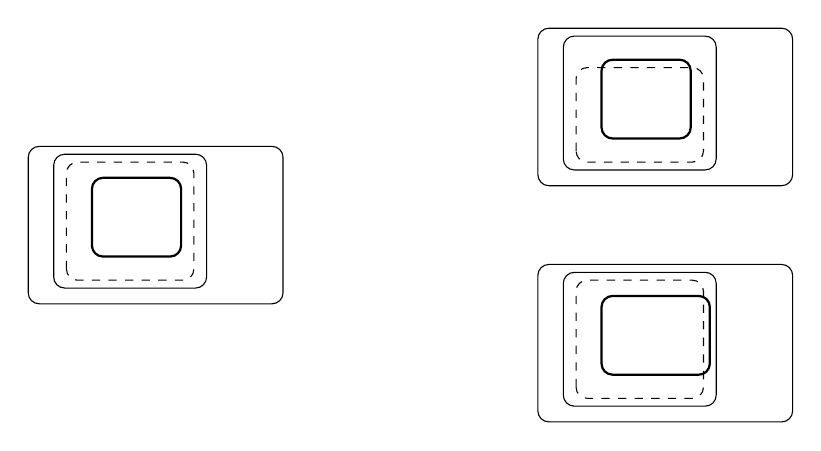
\begin{tikzpicture}
    \pgfmathsetmacro\gr{1.61803}
    \pgfmathsetmacro\by{2}
    \pgfmathsetmacro\bx{\by*\gr}

    \pgfmathsetmacro\pw{\bx*2.5}
    \pgfmathsetmacro\ph{\by*2.5}

    % % % Initial model % % %
    \pgfmathsetmacro\initX{-(\bx)}
    \pgfmathsetmacro\initY{(\ph - \by)/2}

    \draw[rounded corners] (\initX,\initY) rectangle (\initX + \bx,\initY + \by);

    \draw[rounded corners] (\initX +\bx*0.1, \initY + \by*0.1) rectangle (\initX + \bx*0.7,\initY + \by*0.95); % P
    \draw[rounded corners, dashed] (\initX + \bx*0.15,\initY +\by*0.15) rectangle (\initX + \bx*0.65,\initY + \by*0.9);

    \draw[rounded corners, thick] (\initX + \bx*0.25,\initY + \by*0.3) rectangle (\initX + \bx*0.6,\initY + \by*0.8); % Desire

    % % % Slip One % % %
    \pgfmathsetmacro\slipOneX{\bx}
    \pgfmathsetmacro\slipOneY{(\ph - \by)}

    \draw[rounded corners] (\slipOneX,\slipOneY) rectangle (\slipOneX + \bx,\slipOneY + \by);

    \draw[rounded corners] (\slipOneX + \bx*0.1, \slipOneY + \by*0.1) rectangle (\slipOneX + \bx*0.7,\slipOneY + \by*0.95); % P
    \draw[rounded corners, dashed] (\slipOneX + \bx*0.15,\slipOneY + \by*0.15) rectangle (\slipOneX + \bx*0.65,\slipOneY + \by*0.75);

    \draw[rounded corners, thick] (\slipOneX + \bx*0.25, \slipOneY + \by*0.3) rectangle (\slipOneX + \bx*0.6, \slipOneY + \by*0.8); % Desire

    % % % Slip Two % % %
    \pgfmathsetmacro\slipTwoX{\bx}
    \pgfmathsetmacro\slipTwoY{0}

    \draw[rounded corners] (\slipTwoX,\slipTwoY) rectangle (\slipTwoX + \bx,\slipTwoY + \by);

    \draw[rounded corners] (\slipTwoX + \bx*0.1,\slipTwoY + \by*0.1) rectangle (\slipTwoX + \bx*0.7,\slipTwoY + \by*0.95); % P
    \draw[rounded corners, dashed] (\slipTwoX + \bx*0.15,\slipTwoY +\by*0.15) rectangle (\slipTwoX + \bx*0.65,\slipTwoY + \by*0.9);

    \draw[rounded corners, thick] (\slipTwoX + \bx*0.25,\slipTwoY + \by*0.3) rectangle (\slipTwoX + \bx*0.675,\slipTwoY + \by*0.8); % Desire
  \end{tikzpicture}
  \caption{Dynamic slips}
\end{figure}

Conservative with respect to an expression, in the sense that although certain expressions no longer hold relevant significance, the agent's application of the expression can recover the previous instance.
Here we have applicative and desiderative slips.
These terms aren't great, but they sort of work.

But there are also extreme cases of slips, such as when the expression completely slips from the agent's resources.

\begin{figure}[!ht]
  \centering
  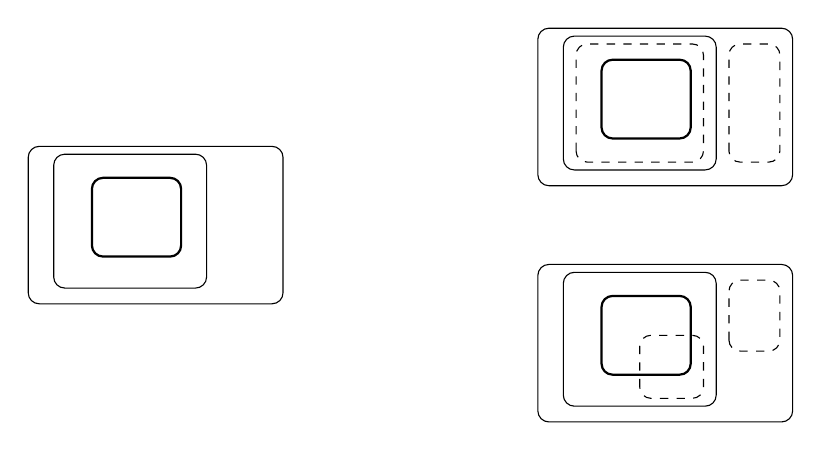
\begin{tikzpicture}
    \pgfmathsetmacro\gr{1.61803}
    \pgfmathsetmacro\by{2}
    \pgfmathsetmacro\bx{\by*\gr}

    \pgfmathsetmacro\pw{\bx*2.5}
    \pgfmathsetmacro\ph{\by*2.5}

    % % % Initial model % % %
    \pgfmathsetmacro\initX{-(\bx)}
    \pgfmathsetmacro\initY{(\ph - \by)/2}

    \draw[rounded corners] (\initX,\initY) rectangle (\initX + \bx,\initY + \by);

    \draw[rounded corners] (\initX +\bx*0.1, \initY + \by*0.1) rectangle (\initX + \bx*0.7,\initY + \by*0.95); % P
    % \draw[rounded corners, dashed] (\initX + \bx*0.15,\initY +\by*0.15) rectangle (\initX + \bx*0.65,\initY + \by*0.9);

    \draw[rounded corners, thick] (\initX + \bx*0.25,\initY + \by*0.3) rectangle (\initX + \bx*0.6,\initY + \by*0.8); % Desire

    % % % Might One % % %
    \pgfmathsetmacro\mightOneX{\bx}
    \pgfmathsetmacro\mightOneY{\ph - \by}

    \draw[rounded corners] (\mightOneX,\mightOneY) rectangle (\mightOneX + \bx,\mightOneY + \by);

    \draw[rounded corners] (\mightOneX + \bx*0.1, \mightOneY + \by*0.1) rectangle (\mightOneX + \bx*0.7,\mightOneY + \by*0.95); % P
    \draw[rounded corners, dashed] (\mightOneX + \bx*0.15,\mightOneY +\by*0.15) rectangle (\mightOneX + \bx*0.65,\mightOneY + \by*0.9);
     \draw[rounded corners, dashed] (\mightOneX + \bx*0.75,\mightOneY +\by*0.15) rectangle (\mightOneX + \bx*0.95,\mightOneY + \by*0.9);


    \draw[rounded corners, thick] (\mightOneX + \bx*0.25, \mightOneY + \by*0.3) rectangle (\mightOneX + \bx*0.6, \mightOneY + \by*0.8); % Desire

    % % % Might Two % % %
    \pgfmathsetmacro\mightTwoX{\bx}
    \pgfmathsetmacro\mightTwoY{0}

    \draw[rounded corners] (\mightTwoX,\mightTwoY) rectangle (\mightTwoX + \bx,\mightTwoY + \by);

    \draw[rounded corners] (\mightTwoX + \bx*0.1,\mightTwoY + \by*0.1) rectangle (\mightTwoX + \bx*0.7,\mightTwoY + \by*0.95); % P
    \draw[rounded corners, dashed] (\mightTwoX + \bx*0.4,\mightTwoY +\by*0.15) rectangle (\mightTwoX + \bx*0.65,\mightTwoY + \by*0.55);
    \draw[rounded corners, dashed] (\mightTwoX + \bx*0.75,\mightTwoY +\by*0.45) rectangle (\mightTwoX + \bx*0.95,\mightTwoY + \by*0.9);

    \draw[rounded corners, thick] (\mightTwoX + \bx*0.25, \mightTwoY + \by*0.3) rectangle (\mightTwoX + \bx*0.6, \mightTwoY + \by*0.8); % Desire
  \end{tikzpicture}
  \caption{Dynamic might}
\end{figure}

Here we suppose that the agent doesn't do anything with some expression.
Two uses of `might'.
First, to update the agent's application of an expression.
Second, to describe the result.
With the update, things can go well, when describing we typically have the bad case in mind.

Could also float the idea of a desiderative might.
So, forming the means for something which may of may not satisfy the agent.
This is the ice cream style example.
Certain abuse of the model is required here.
As need to pick some arbitrary collection of situations, something that the agent doesn't have the resources to evaluate.
But I think this is fine, because the guiding interpretation is that the attentive component is enough to evaluate.
That is, there are still the truth values hanging about, and hence the agent can do something with these, even if they don't know how to evaluate them.




These are the two key dynamics we need.
First there's a fixed `slip', then there's a successful might.
At least, this is all that's needed from a very general perspective.
What we haven't captured is the way that the means help recover the end.

Here is where belief becomes important.
Basically, belief picks out a subset of situations, using the fact that you want to hear the song again.
Then, you lose the information and your belief expands.
You then rule out certain situations.
And eventually there's a might again.





\begin{figure}[ht]
  \centering
  \begin{subfigure}[b]{0.3\textwidth}
    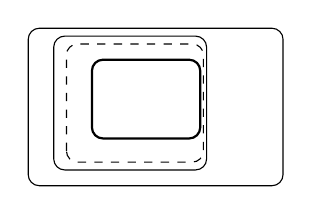
\begin{tikzpicture}
      \pgfmathsetmacro\gr{1.61803}
      \pgfmathsetmacro\by{2}
      \pgfmathsetmacro\bx{\by*\gr}
      \draw[rounded corners] (0,0) rectangle (\bx,\by);

      \draw[rounded corners] (\bx*0.1, \by*0.1) rectangle (\bx*0.7,\by*0.95); % P

      \draw[rounded corners, dashed] (\bx*0.15,\by*0.15) rectangle (\bx*0.6875,\by*0.9);

      \draw[rounded corners, thick] (\bx*0.25, \by*0.3) rectangle (\bx*0.675,\by*0.8); % Desire
    \end{tikzpicture}
    \caption{Both}
  \end{subfigure}
\end{figure}




\begin{figure}[ht]
  \centering
  \begin{subfigure}[b]{0.3\textwidth}
    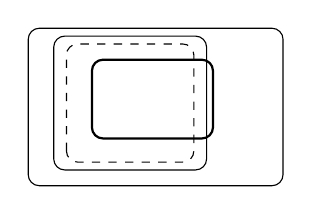
\begin{tikzpicture}
      \pgfmathsetmacro\gr{1.61803}
      \pgfmathsetmacro\by{2}
      \pgfmathsetmacro\bx{\by*\gr}
      \draw[rounded corners] (0,0) rectangle (\bx,\by);

      \draw[rounded corners] (\bx*0.1, \by*0.1) rectangle (\bx*0.7,\by*0.95); % P

      \draw[rounded corners, dashed] (\bx*0.15,\by*0.15) rectangle (\bx*0.65,\by*0.9);

      \draw[rounded corners, thick] (\bx*0.25, \by*0.3) rectangle (\bx*0.725,\by*0.8); % Desire
    \end{tikzpicture}
    \caption{Difficult}
  \end{subfigure}
  \caption{Three different `updates'}
\end{figure}



\newpage


\section{Logic Notes}
\label{sec:logic-notes}

\begin{proposition}
  The up and down versions of mental operators are not interdefinable.
  \begin{proof}
    Consider \(\ldesd{p} \rightarrow \lnot p\).

    Suppose a frame is not irreflexive. Then, value the relflexive point \(p\), and the formula is false at this point.

    Conversely, suppose the formula is invalid.
    Then \(\ldesd{p} \land p\) for some point, which means that this point must be accessible from itself, and hence the frame cannot be irreflexive.
  \end{proof}
\end{proposition}


\begin{example}
  The two sub-consequence relations are distinct.
  For example: \(p \lint q \vDash \ast, q\), but \(p \lint q \nvDash q\).
  {\color{red} It's not clear that this kind of thing holds for classical logical operators.}
\end{example}



\subsection{Sequential Rules}
\label{sec:sequential-rules}

\subsubsection{Structural Rules}
\label{sec:structural-rules}

four structural rules, more or less standard.

\begin{prooftree}
  \def\fCenter{\mbox{\ \(\cap\)\ }}
  \Axiom\(\Gamma \fCenter\ \Delta \ne \emptyset\)
  \RightLabel{(Start)}
  \def\fCenter{\mbox{\ \(\seq\)\ }}
  \UnaryInf\(\Gamma \fCenter\ \Delta\)
\end{prooftree}



\begin{multicols}{2}
  \begin{prooftree}
    \def\fCenter{\mbox{\ \(\seq\)\ }}
    \Axiom\(\Gamma \fCenter\ \Delta\)
    \def\fCenter{\mbox{\ \(\subseteq\)\ }}
    \Axiom\(\Delta \fCenter\ \Delta'\)
    \RightLabel{(R-Mon)}
    \def\fCenter{\mbox{\ \(\seq\)\ }}
    \BinaryInf\(\Gamma \fCenter\ \Delta'\)
  \end{prooftree}

\begin{prooftree}
  \def\fCenter{\mbox{\ \(\seq\)\ }}
  \Axiom\(\Gamma \fCenter\ \Delta\)
  \def\fCenter{\mbox{\ \(\subseteq\)\ }}
  \Axiom\(\Gamma \fCenter\ \Gamma'\)
  \RightLabel{(L-Mon)}
  \def\fCenter{\mbox{\ \(\seq\)\ }}
  \BinaryInf\(\Gamma' \fCenter\ \Delta\)
\end{prooftree}
\end{multicols}

\begin{prooftree}
  \def\fCenter{\mbox{\ \(\seq\)\ }}
  \Axiom\(\Gamma, \phi \fCenter \Delta\)
  \Axiom\(\Gamma \fCenter \phi, \Delta\)\RightLabel{(Cut)}
  \BinaryInf\(\Gamma \fCenter \Delta\)
\end{prooftree}

\subsubsection{Propositional rules}
\label{sec:propositional-rules}

Collection of general propositional rules which are valid for any type of formula.

\begin{multicols}{2}
  \begin{prooftree}
    \def\fCenter{\mbox{\ \(\seq\)\ }}
    \AxiomC{}
    \UnaryInfC{\(\fCenter \top\)}
  \end{prooftree}

  \begin{prooftree}
    \def\fCenter{\mbox{\ \(\seq\)\ }}
    \AxiomC{}
    \UnaryInfC{\(\bot \fCenter\)}
  \end{prooftree}
\end{multicols}

\begin{multicols}{2}
  \begin{prooftree}
    \def\fCenter{\mbox{\ \(\seq\)\ }}
    \AxiomC{}
    \UnaryInfC{\(\lnot\ast \fCenter \ast\)}
  \end{prooftree}

  \begin{prooftree}
    \def\fCenter{\mbox{\ \(\seq\)\ }}
    \AxiomC{}
    \UnaryInfC{\(\ast \fCenter \lnot\ast\)}
  \end{prooftree}
\end{multicols}

\begin{multicols}{2}
  \begin{prooftree}
    \def\fCenter{\mbox{\ \(\seq\)\ }}
    \AxiomC{}
    \UnaryInfC{\(\phi,\lnot\phi \fCenter \ast\)}
  \end{prooftree}

  \begin{prooftree}
    \def\fCenter{\mbox{\ \(\seq\)\ }}
    \AxiomC{}
    \UnaryInfC{\(\ast \fCenter \phi,\lnot\phi\)}
  \end{prooftree}
\end{multicols}


\begin{multicols}{2}
  \begin{prooftree}
  \def\fCenter{\mbox{\ \(\seq\)\ }}
  \Axiom\(\lnot\Gamma \fCenter \Delta\)
  \UnaryInf\(\lnot\Delta \fCenter \Gamma\)
\end{prooftree}
\columnbreak

\begin{prooftree}
  \def\fCenter{\mbox{\ \(\seq\)\ }}
  \Axiom\(\Gamma \fCenter\ \lnot\Delta\)
  \UnaryInf\(\Delta \fCenter\ \lnot\Gamma\)
\end{prooftree}
\end{multicols}

\begin{multicols}{2}
  \begin{prooftree}
    \def\fCenter{\mbox{\ \(\seq\)\ }}
    \Axiom\(\Gamma,\phi,\psi \fCenter\ \Delta\)
    \doubleLine
    \UnaryInf\(\Gamma,\phi\land\psi \fCenter\ \Delta\)
  \end{prooftree}

  \begin{prooftree}
    \def\fCenter{\mbox{\ \(\seq\)\ }}
    \Axiom\(\Gamma \fCenter\ \phi,\psi \Delta\)
    \doubleLine
    \UnaryInf\(\Gamma \fCenter\ \phi\lor\psi, \Delta\)
  \end{prooftree}
\end{multicols}


\begin{multicols}{2}
  \begin{prooftree}
    \def\fCenter{\mbox{\ \(\seq\)\ }}
    \Axiom\(\Gamma,\phi,\psi \fCenter\ \ast, \Delta\)
    \doubleLine
    \UnaryInf\(\Gamma,\phi\lint\psi \fCenter\ \ast, \Delta\)
  \end{prooftree}

  \begin{prooftree}
    \def\fCenter{\mbox{\ \(\seq\)\ }}
    \Axiom\(\Gamma,\ast \fCenter\ \phi,\psi, \Delta\)
    \doubleLine
    \UnaryInf\(\Gamma,\ast \fCenter\ \phi\lint\psi, \Delta\)
  \end{prooftree}
\end{multicols}

These are supplemented with two collections of special rules.
One for partial propositions and the other for total propositions.

For partial propositions we ensure consistency with a pair of fairly heavy-handed rules.
Note these are not hold in both directions.

\begin{multicols}{2}
  \begin{prooftree}
    \def\fCenter{\mbox{\ \(\seq\)\ }}
    \Axiom\(\Gamma,\attn{\phi} \fCenter\ \Delta\)
    \UnaryInf\(\Gamma,\attn{\phi},\phi \fCenter\ \Delta\)
  \end{prooftree}

  \begin{prooftree}
    \def\fCenter{\mbox{\ \(\seq\)\ }}
    \Axiom\(\Gamma \fCenter\ \attn{\phi}, \Delta\)
    \UnaryInf\(\Gamma \fCenter\ \attn{\phi} \land \phi, \Delta\)
  \end{prooftree}
\end{multicols}




\subsubsection{Modal Rules}
\label{sec:modal-rules}

Following \citeauthor{Jaspars:1996aa}, we introduce a single rule covering the general semantics of box-type formulas in our system.
This rule is termed general as it does not depend on the constraints we place on accessibility relations.

\begin{prooftree}
  \def\fCenter{\mbox{\ \(\seq\)\ }}
  \Axiom\(\Gamma \fCenter\ \phi, \lnot\Delta\)
  \RightLabel{(Box-1)}
  \UnaryInf\(\Box\Gamma \fCenter\ \Box\phi, \lnot\Box\Delta\)
\end{prooftree}

\begin{lemma}[Soundness]
  The general modal rule is sound.
  \begin{proof}
    Suppose \(\Gamma,\lnot\phi \vdash \lnot\Delta\).

    For the left-to-right sub-consequence relation. And, suppose \(\Box\Gamma, \lnot\Box\phi\) holds at some world. Then, some world at which \(\lnot\phi\) is true along with \(\gamma \in \Gamma\), but then at this world some \(\delta \in \Delta\) must fail to hold, and hence \(\lnot\Box\Delta\).

    For the right-to-left sub-consequence relation. Suppose \(\Box\Delta\). Then, take any world, if no world then \(\Box\phi\), and if some world then either \(\phi\) is true at all, and hence \(\Box\phi\), or some \(\gamma \in \Gamma\) is false, and hence not \(\Box\Gamma\).
  \end{proof}
\end{lemma}

While \citeauthor{Jaspars:1996aa} also require the contrapositive of (Box-1), we can derive this.

\begin{proposition}
  The following rule is derivable in our system.
    \begin{prooftree}
  \def\fCenter{\mbox{\ \(\seq\)\ }}
  \Axiom\(\Gamma,\lnot\phi \fCenter\ \lnot\Delta\)
  \RightLabel{(Box-2)}
  \UnaryInf\(\Box\Gamma,\lnot\Box\phi \fCenter\ \lnot\Box\Delta\)
\end{prooftree}
  \begin{proof}
    By applying the contraposition rule, changing variables used.
  \end{proof}
\end{proposition}

Window-type modalities are governed by a corresponding rule.

    \begin{prooftree}
    \def\fCenter{\mbox{\ \(\seq\)\ }}
    \Axiom\(\Gamma \fCenter\ \phi, \lnot\Delta\)
    \RightLabel{(Window-1)}
    \UnaryInf\(\Window\Gamma \fCenter\ \Window\lnot\phi, \Window\Delta\)
  \end{prooftree}


\begin{proposition}[Finiteness]
  If \(\Gamma \vdash \Delta\) then there exist finite \(\Gamma' \subseteq \Gamma\) and \(\Delta' \subseteq \Delta\) such that \(\Gamma' \vdash \Delta'\).
  \begin{proof}
    By induction on the length of proofs.
    Base cases show how to find the finite sets, and then the rules only manipulate finite subsets.
  \end{proof}
\end{proposition}


\subsection{Completeness Ideas}
\label{sec:completeness-ideas}

Completeness follows the traditional path of showing how to construct a countermodel for any failure of derivability.
The structural rule (T) is important here.
For, if \(\Gamma \nvdash \Delta\), then (T) guarantees there is no \(\lambda\) such that \(\Gamma,\lambda \vdash \Delta\) and \(\Gamma \vdash \lambda,\Delta\).
Spelt out, this means that there's no expression \(\lambda\) which connects \(\Gamma\) and \(\Delta\) by requiring that when every expression in \(\Gamma\) is true then some expression in \(\Delta\) must also be true and if every expression in \(\Delta\) is false then some expression in \(\Gamma\) is false.
Hence, it will be possible to expand \(\Gamma\) and \(\Delta\) to an exhaustive pair \(\Gamma'\) and \(\Delta'\) partitioning the language, which in turn will provide the basis for specifying a countermodel.



The exhaustive pair specifies a point.

\begin{note}
  The basic idea is to take pairs of formulas. The pairs of interest are those in which the consequence relation does not trivially hold. Due to there being two directions to consider, this requires keeping track of which direction is of interest. If these pairs were finite, we could potentially focus on one direction, but as these may be infinite, we can't appeal to the rule of contraposition in the proof system.

  The goal is to take any consistent pair, and show that it can be made exhaustive. These exhaustive pairs will then form the basis for the canonical model.

  Conjecture: Only one of the pairs is required, as any given pair can be flipped through negation. However, it's not clear that this can easily be proven prior to the truth lemma, which is what's grounding the intuition.
\end{note}





\begin{proposition}\label{prop:finiteness}
  \(\Gamma \vDash \Delta\) iff \(\Gamma \vDash \ast, \Delta\) and \(\Gamma, \ast \vDash \Delta\).
  \begin{proof}
    From left to right, if the entailment holds, then it's got to be the case that the weakenings hold.
And, from right to left, this relies on the relevant definitions to show that the respective instances of \(\ast\) can be eliminated.
  \end{proof}
\end{proposition}

This allows us to split the consequence relation.
The use of this is to observe that there only needs to be one sub-failure of entailment.
This is, in part, what motivates the idea of taking exhaustive pairs.
For if \(\Gamma \nvdash \Delta\) then it must be the case that adding \(\ast\) to one of the sides preserves the failure.
Hence, we can potentially weaken while preserving the failure.
And, we don't need to directly deal with both sub-instances of entailment.





\begin{definition}[Consistency]
  Consistency is a mix of two conditions, because of the double-barrelled consequence relation.
  And, \(\ast\) is used this separates the two conditions.
  If a contradiction were used, this would lead to a stronger condition.
  \begin{itemize}
  \item \(\Gamma\) is consistent iff \(\Gamma \nvdash \ast\) or \(\ast \nvdash \Gamma\).
  \item \(\opair{\Gamma}{\Delta}\) is consistent iff either \(\Gamma\) or \(\Delta\) is consistent.
    \begin{itemize}
    \item Left consistency and right consistency, respectively.
    \end{itemize}
  \end{itemize}
  It turns out that either or the two conditions for consistency can be used, as a valuation for one condition can be inverted to provide a valuation for the other.
\end{definition}

Consistent sets will be saturated, and correspond to states.

The idea of saturation is key, but the double-barrelled notion of consequence requires some generalisations, as we may need to saturate for either truth or falsity.
\cite{Thomason:1968aa} and \cite{Aczel:1968aa} provide the foundations for saturated theories.

\begin{definition}[Saturation]
  Given a set of formulas \(\Gamma\), we say that \(\Gamma\) is:
  \begin{itemize}
  \item left-saturated if for all \(\Sigma\), if \(\Gamma \vdash \ast, \Sigma\) then \(\Gamma \cap \Sigma \ne \emptyset\)
  \item right-saturated if for all \(\Sigma\), if \(\Sigma, \ast \vdash \Gamma\) then \(\Gamma \cap \Sigma \ne \emptyset\)
  \end{itemize}
\end{definition}

Note that these dual notions of saturation correspond to the two notions of consistency.

\begin{definition}[Saturators]
  \mbox{ }
  \begin{itemize}
  \item \(\Lambda\) is a left saturator of \(\Gamma\) iff for all \(\Delta\) if \(\Gamma \vdash \ast, \Delta\) then \(\Delta \cap \Lambda \ne \emptyset\)
  \item \(\Lambda\) is a right saturator of \(\Gamma\) iff for all \(\Delta\) if \(\Delta, \ast \vdash \Gamma\) then \(\Delta \cap \Lambda \ne \emptyset\)
  \end{itemize}
\end{definition}


The Lindenbaum lemma is move involved than usual.
A saturated pair is either left or right saturated.
However, it may be possible for a pair to be either left or right saturated.
For example, \(\opair{\{p\}}{\{q\}}\).
Here, there are two exhaustive pairs, both of which would be fit for purpose.
Instead of choosing, we introduce two cases of saturation.



For left saturation, we immediately introduce an \(\ast\) on the right.
This weakens the consequence relation, as desired.

\begin{lemma}[Lindenbaum, left]\label{lindenbaum:left}
  Suppose \(\Lambda\) is a left saturator of \(\opair{\Gamma}{\Delta}\), then there's a left-saturated exhaustive pair \(\opair{\Gamma^{+}}{\Delta^{+}}\) such that \(\Gamma \subseteq \Gamma^{+} \subseteq \Lambda\).


  \begin{proof}
    Let \(\{\phi\}_{i_{i \in \omega}}\) be an enumeration of \(\olang{}\) such that every element of \(\Lambda\) occurs infinitely many times.\nolinebreak

    Given \(\{\phi\}_{i \in \omega}\), we define a sequence \(\opair{\Gamma_{i}}{\Delta_{i}}_{i \in \omega}\) such that \(\Lambda\) is a left-saturator of each \(\opair{\Gamma_{i}}{\Delta_{i}}\), with the limit of the sequence providing the desired left-saturated pair \(\opair{\Gamma^{+}}{\Delta^{+}}\).

    \begin{align*}
      \opair{\Gamma_{0}}{\Delta_{0}} &= \opair{\Gamma}{\Delta \cup \{\ast\}} \\
      \opair{\Gamma_{n+1}}{\Delta_{n+1}} &=
                                                  \begin{cases}
                                                    \opair{\Gamma_{n} \cup \{\phi_{n}\}}{\Delta_{n}} &\text{if for all finite } \Sigma \colon  \\
                                                    &\quad \Sigma \cap \Lambda \ne \emptyset, \text{ when } \Gamma_{n},\phi_{n} \vdash \ast, \Sigma \\
                                                    \opair{\Gamma_{n}}{\Delta_{n} \cup \{\phi_{n}\}}
                                                    &\text{otherwise} \\
                                                  \end{cases}
      \\
      \opair{\Gamma^{+}}{\Delta^{+}} &= \opair{\bigcup_{n \in \omega}\Gamma_{n}}{\bigcup_{n\in\omega}\Delta_{n}}
    \end{align*}
    Note first that \(\opair{\Gamma^{+}}{\Delta^{+}}\) is exhaustive by construction.

    To see that \(\Gamma^{+} \subseteq \Lambda\) note that by definition:
    \begin{enumerate}[label=(\arabic*)]
    \item\label{leftLindenbaum:1} if \(\Gamma_{n} \vdash \ast, \Sigma\) then \(\Sigma \cap \Lambda \ne \emptyset\) for all finite \(\Sigma \subseteq \olang{}\).
    \end{enumerate}
    By proposition~\ref{prop:finiteness} this means that \(\Lambda\) is a saturator of each \(\Gamma_{n}\), and so by some other observation we have \(\Gamma^{+} \subseteq \Lambda\).

    To establish the left-saturation of \(\opair{\Gamma^{+}}{\Delta^{+}}\) we show that:
    \begin{enumerate}[label=(\arabic*),resume]
    \item\label{leftLindenbaum:2} For all \(k \in \omega \colon\) if \(\Gamma_{k} \vdash \ast, \Sigma\) and \(\Sigma\) is finite, then \(\Sigma \cap \Gamma^{+} \ne \emptyset\).
    \end{enumerate}

    This is where the repeated instances of a proposition in the enumeration \(\{\phi_{i}\}_{i \in \omega}\) comes into play.
    For, suppose that for some \(k\) and finite \(\Sigma\) it is the case that \(\Gamma_{k} \vdash \ast, \Sigma\) but \(\Sigma \cap \Gamma^{+} = \emptyset\).
    By \ref{leftLindenbaum:1} we know that \(\Sigma \cap \Lambda\) is non-empty, and as each formula occurs in \(\{\phi_{i}\}_{i \in \omega}\) infinitely many times let \(\{\phi_{k_{1}}, \dots, \phi_{k_{n}}\}\) be an enumeration of \(\Sigma \cap \Lambda\) such that \(k < k_{i}\) for all \(i\) and \(k_{i} < k_{j}\) for \(i < j\).
    Intuitively, the enumeration \(\{\phi_{k_{1}}, \dots, \phi_{k_{n}}\}\) identifies some instance of each \(\phi \in \Sigma \cap \Lambda\) which are yet to be considered at the \(k^{\text{th}}\) stage of the sequence.

    For each \(\phi_{k_{i}}\) it must be that \mbox{\(\Gamma, \phi_{k_{i}} \vdash \ast, \Sigma_{i}\)} for some finite \(\Sigma_{i}\) such that \(\Sigma_{i} \cap \Lambda = \emptyset\), by the construction of \(\Gamma^{+}\).

    Still, \mbox{\(\Gamma_{k} \vdash \ast, \Sigma\)}, and so in particular \mbox{\(\Gamma_{k} \vdash \ast, \phi_{k_{i}},\Sigma - \{\phi_{k_{i}}\}\)} for each \(\phi_{k_{i}}\).
    Consider \mbox{\(\Gamma_{k} \vdash \ast, \phi_{k_{1}},\Sigma - \{\phi_{k_{1}}\}\)} and note that \mbox{\(\Gamma_{k_{1}}, \phi_{k_{1}} \vdash \ast, \Sigma_{1}\)}.
    From the latter two observations and an instance of Cut we obtain \mbox{\(\Gamma_{k}, \Gamma_{k_{1}} \vdash \ast, \Sigma - \{\phi_{k_{1}}\}, \Sigma_{1}\)}.
    And, as \mbox{\(\Gamma_{k} \subseteq \Gamma_{k_{1}}\)}, we can infer that \mbox{\(\Gamma_{k_{1}} \vdash \ast, \Sigma - \{\phi_{k_{1}}\}, \Sigma_{1}\)}.

    The previous steps can be replicated for each \(\phi_{k_{i}}\), noting that \(\Gamma_{k_{i}} \subseteq \phi_{k_{i+1}}\), from which we obtain \mbox{\(\Gamma_{k_{n}} \vdash \ast, \Sigma - \{\phi_{k_{1}},\dots,\phi_{k_{n}}\}, \Sigma_{1},\dots,\Sigma_{n}\)}.
    As \(\Sigma\) is finite by assumption, and each \(\Sigma_{i}\) is also finite (of which there are a finitely many), this means the union of the sets of the right hand side of the consequence relation is finite.
    Yet, \((\Sigma - \{\phi_{k_{1}},\dots,\phi_{k_{n}}\} \cup \Sigma_{1} \cup \dots \cup \Sigma_{n}) \cap \Lambda = \emptyset\), contradicting \ref{leftLindenbaum:1}, above.

    So, for any finite \(\Gamma_{k}\), if \(\Gamma_{k} \vdash \ast, \Sigma\) and \(\Sigma\) is finite, then \(\Sigma \cap \Gamma^{+} \ne \emptyset\).

    By proposition~\ref{prop:finiteness}, if \(\Gamma^{+} \vdash \ast, \Sigma\) then there are finite subsets \(\Gamma \subseteq \Gamma^{+}\) and \(\Sigma' \subseteq \Sigma\) such that \(\Gamma \vdash \ast, \Sigma\) and by construction of \(\Gamma^{+}\) there is some \(n \in \omega\) such that \(\Gamma_{n} \vdash \ast, \Sigma'\).
    From \label{leftLindenbaum:2} we know that \(\Sigma' \cap \Gamma^{+} \ne \emptyset\) and so \(\Sigma \cap \Gamma^{+} \ne \emptyset\).
    Therefore, \(\opair{\Gamma^{+}}{\Delta^{+}}\) is left-saturated.
  \end{proof}

\end{lemma}

For right saturation, we move our attention to the right-to-left sub-consequence relation.

\begin{lemma}[Lindenbaum, right]\label{lindenbaum:right}
  Suppose \(\Lambda\) is a right saturator of \(\opair{\Gamma}{\Delta}\), then there's a right-saturated pair \(\opair{\Gamma^{+}}{\Delta^{+}}\) such that \(\Delta \subseteq \Delta^{+} \subseteq \Lambda\).
  \begin{proof}
    The proof strategy for right-saturation is analogous to left-saturation, altered only for the corresponding change in sub-consequence relation of interest.
    \begin{align*}
      \opair{\Gamma_{0}}{\Delta_{0}} &= \opair{\Gamma \cup \{\ast\}}{\Delta} \\
      \opair{\Gamma_{n+1}}{\Delta_{n+1}} &=
                                                  \begin{cases}
                                                    \opair{\Gamma_{n}}{\Delta_{n} \cup \{\phi_{n}\}} &\text{if for all finite } \Sigma \colon\\
                                                    &\quad \Sigma \cap \Lambda \ne \emptyset, \text{ when } \Sigma,\ast \vdash \phi_{n},\Delta_{n} \\
                                                    \opair{\Gamma_{n} \cup \{\phi_{n}\}}{\Delta_{n}} &\text{otherwise} \\
                                                  \end{cases}
      \\
      \opair{\Gamma^{+}}{\Delta^{+}} &= \opair{\bigcup_{n \in \omega}\Gamma_{n}}{\bigcup_{n\in\omega}\Delta_{n}}
    \end{align*}
    Again, \(\opair{\Gamma^{+}}{\Delta^{+}}\) is exhaustive by construction and the following two properties can be established:
    \begin{enumerate}[label=(\arabic*)]
    \item\label{rightLindenbaum:1} If \(\Sigma,\ast \vdash \Delta_{n}\) then \(\Sigma \cap \Lambda \ne \emptyset\) for all finite \(\Sigma\).
    \item\label{rightLindenbaum:2} For all \(k \in \omega \colon\) if \(\Sigma, \ast \vdash \Delta_{k}\) and \(\Sigma\) is finite, then \(\Sigma \cap \Delta^{+} \ne \emptyset\).
    \end{enumerate}
  \end{proof}
\end{lemma}



\begin{corollary}[Saturation]
  If \(\Gamma \nvdash \Delta\) then there exists an exhaustive pair \(\opair{\Gamma^{+}}{\Delta^{+}}\) such that \(\Gamma^{+} \cap \Delta^{+} = \emptyset\) with \(\Gamma \subseteq \Gamma^{+}\) and \(\Delta \subseteq \Delta^{+}\) and either
  \begin{enumerate}
  \item If \(\Gamma \nvdash \ast, \Delta\) then \(\opair{\Gamma^{+}}{\Delta^{+}}\) is a left-saturated pair, or
  \item If \(\Gamma,\ast \nvdash \Delta\) then \(\opair{\Gamma^{+}}{\Delta^{+}}\) is a right-saturated pair.
  \end{enumerate}
  \begin{proof}
    If \(\Gamma \nvdash \Delta\) then either \(\Gamma \nvdash \ast, \Delta\) or \(\Gamma, \ast \nvdash \Delta\).

    Suppose \(\Gamma \nvdash \ast, \Delta\).
    Then, \(\Delta^{c} = \olang{} - \Delta\) is a left-saturator of \(\olang{\Gamma}{\Delta}\).
    For, \(\Delta^{c}\) is \emph{not} a saturator of \(\Gamma\) if and only if there is some \(\Sigma\) such that \(\Gamma \vdash \ast, \Sigma\) with \(\Sigma \cap \Delta^{c} = \emptyset\).
    Yet, if \(\Sigma \cap \Delta^{c} = \emptyset\), then \(\Sigma \subseteq \Delta\), and so by R-Mon the previous is the case if and only if \(\Gamma \vdash \ast, \Delta\) contradicting our initial assumption.

    So, as \(\Delta^{c}\) is a left-saturator of \(\opair{\Gamma}{\Delta}\) and appeal to lemma~\ref{lindenbaum:left} ensures there is a left-saturated pair \(\opair{\Gamma^{+}}{\Delta^{+}}\) such that \(\Gamma \subseteq \Gamma^{+} \subseteq \Delta^{c}\) and hence \(\Gamma^{+} \cap \Delta = \emptyset\).

    Likewise, if \(\Gamma, \ast \nvdash \Delta\) then \(\Gamma^{c}\) is a right-saturator of \(\olang{\Gamma}{\Delta}\) we appeal to lemma~\ref{lindenbaum:right} to find a right-saturated pair \(\opair{\Gamma^{+}}{\Delta^{+}}\) with the desired properties.
  \end{proof}
\end{corollary}

\begin{lemma}[Correspondence]\label{lem:correspondence}
  \(\olang{\Gamma}{\Delta}\) is left-saturated iff \(\opair{\lnot\Delta}{\lnot\Gamma}\) is right-saturated.
  \begin{proof}
    From left to right, if \(\olang{\Gamma}{\Delta}\) is left-saturated then, for finite \(\Sigma\), whenever \(\Gamma \vdash \Sigma\), \(\Gamma \cap \Sigma \ne \emptyset\).
    Suppose for some finite \(\Sigma'\), \(\Sigma' \vdash \lnot\Gamma\).
    Then, \(\Gamma \vdash \lnot\Sigma'\), by {\color{red} the rule}.
    However, by the above this means that \(\Gamma \cap \lnot\Sigma' \ne \emptyset\), from which it follows that \(\lnot\Gamma \cap \Sigma' \ne \emptyset\), as if \(\phi \in \Gamma \cap \lnot\Sigma'\) then \(\phi \in \Gamma\) and \(\phi \in \lnot\Sigma'\) which ensures that \(\lnot\phi \in \lnot\Gamma\) and \(\lnot\phi \in \Sigma'\).
  \end{proof}
\end{lemma}

Lemma~\ref{lem:correspondence} shows that lemmas~\ref{lindenbaum:left} and~\ref{lindenbaum:right} amount to the same thing, and either can be indirectly used to prove the other.\nolinebreak
\footnote{This is a version of \citeauthor{Blamey:1980aa}'s Lemma III.2.15 (\citeyear[122]{Blamey:1980aa})}
However, the primary use of lemma~\ref{lem:correspondence} will be to simplify our canonical model.
For, instead of taking saturated pairs in general, we may take either left- or right-saturated pairs without loss of generality, reducing the number of cases we need to consider when establishing the relevant truth lemma.


\subsection{The Caonical Model}
\label{sec:caonical-model}


\begin{definition}[Canonical Model]
  \(\cmodel = (W,R^{+},R^{-},V)\) where:
  \begin{itemize}
  \item \(W\) is the set of all saturated sets.
  \item \(\)
  \end{itemize}
  
  Here, take only left-saturated pairs.
\end{definition}

\begin{lemma}
  For any \(\opair{\Gamma}{\Delta}\), \(\opair{\Xi}{\Psi}\) in \(W\).
  \begin{itemize}
  \item If \(\Box^{-}\Gamma \subseteq \Xi\) then there exists a \(\Xi' \subseteq \Xi\) such that \(\opair{\Gamma}{\Delta} R \opair{\Xi'}{\Psi'}\)
  \item If \(\Box^{-}\Gamma \subseteq \Psi\) then there exists a \(\Psi' \subseteq \Psi\) such that \(\opair{\Gamma}{\Delta} R \opair{\Xi'}{\Psi'}\)
  \end{itemize}
\end{lemma}



The truth lemma is split into a pair of truth lemmas, corresponding to the two sub-cases of consequence.
Key here is that the presence of \(\ast\) on the left or right determines which of a pair is taken.



\begin{lemma}[Truth, left]
  \(\Gamma \vDash \phi\) iff \(\phi \in \Gamma\) and \(\Gamma \Dashv \phi\) iff \(\lnot\phi \in \Gamma\)
\end{lemma}

\begin{lemma}[Truth, right]
  \(\Delta \vDash \phi\) iff \(\lnot\phi \in \Delta\) and \(\Delta \Dashv \phi\) iff \(\phi \in \Delta\)
\end{lemma}


\newpage


\begin{definition}\mbox{ }
  \begin{itemize}
  \item K: \(\Box(\phi \land \psi) \rightarrow (\Box\phi \land \Box\psi)\)
  \item D: \(\lnot\Box\bot\)
  \item 4: \(\Box\phi \rightarrow \Box\Box\phi\)
  \item 5: \(\lnot\Box\phi \rightarrow \Box\lnot\Box\phi\)
  \end{itemize}
\end{definition}

\subsection{Frame Conditions}
\label{sec:frame-conditions}

Want: \(K45\) for each of the modal operators.
That is, the operator identifies a set/equivalence relation for any accessible state.
\(D\) should be omitted in general case, but some non-triviality condition should be able to be assumed.

{\color{red} Question: Is there an implicit quantifier that these formulas hold for all formulas?
  If so, the restriction is only going to come of the left hand side, and so specifying the counterexample with respect to an atomic formula will be fine.
And, as the right to left direction doesn't depend on bivalence, this should work too.}

\begin{proposition}[Transitivity]
  \(\oframe{F} \vDash \Box\phi \rightarrow \Box\Box\phi\) iff \(\oframe{F}\) is transitive.
  \begin{proof}
    Take an arbitrary model based on a transitive frame \(\oframe{F}\).
    Suppose \(\Box\phi\) but \(\lnot\Box\Box\phi\).
    Some \(t,u\) such that \(Rst\) and \(Rtu\) but \(t \nvDash \phi\).
    However, from this it follows that \(Rsu\) and it must be the case that \(t \vDash \phi\).

    Conversely, take a non-transitive frame and value the \(u\) point as the only one where \(\phi\) is false, and let the rest of the valuation be determined by what \(\phi\) requires (or, rather, perhaps this only needs to hold for propositional atoms\dots).
  \end{proof}
\end{proposition}

\begin{proposition}
  \(\oframe{F} \vDash \lnot\Box\phi \rightarrow \Box\lnot\Box\phi\) iff \(\oframe{F}\) is euclidean.
  \begin{proof}
    Suppose the frame is euclidean but for some valuation the formula isn't valid.
    Then, \(s \vDash \lnot\Box\phi\) and \(s \nvDash \Box\lnot\Box\phi\).
    So, some accessible state \(t\) such that \(t \nvDash \phi\).
    And, \(s \nvDash \Box\lnot\Box\phi\) so \(s \vDash \Diamond\Box\phi\).
    Hence, some \(u\) such that \(u \vDash \Box\phi\).
    But then as the frame is euclidean, it's got to be the case that \(Rut\), hence \(t \nvDash \phi\) and \(t \vDash \phi\).

    Conversely, valuation such that \(t\) is the only state that doesn't make \(\phi\) true.
  \end{proof}
\end{proposition}

\begin{note}
  \([U]A \coloneq N(A,A) \coloneq \Box A \land H \lnot A\).
  Ah, this means that \(A\) holds everywhere.
  For, if \(\Box A\) then it must be the case that \(S \subseteq \sem{A}\).
  And, if \(H A\) then it must be the case that \(\sem{\lnot A} \subseteq S\).
  But, if \(\sem{\lnot A} \ne \emptyset\) then it'd be the case that \(\sem{A} \cap \sem{\lnot A} \ne \emptyset\), which is impossible.
\end{note}

So, basic strategy for completeness is to move to the kind of model where for each pair of metal operators, there are two relations which are exclusive of one another, noting a one-to-one correspondence between these models and the kind I'm interested in.
Completeness then proceeds through these `generalised' models.



\section{Canonical Model}
\label{sec:canonical-model}

On generalised models, \citeauthor{Gargov:1987aa} give a revised definition of the window modality.

\begin{itemize}
\item \(s \vDash B\phi\) iff \(\forall t(Rst \rightarrow t \vDash \phi)\)
\item \(s \vDash W\phi\) iff \(\forall t(t \vDash \phi \rightarrow \lnot Sst)\)
\end{itemize}

Where \(s \vDash W\phi\) iff \(\forall t(t \vDash \phi \rightarrow Rst)\) is standard.

The general idea here seems sound for generalising.
For the \(W\) modality, I have \(\forall t(\lnot Rst \rightarrow t \vDash \lnot\phi)\).
Given this, I may want something else.
Perhaps, \(s \vDash W\phi \) iff \(\forall t(Sst \rightarrow t \vDash \lnot\phi)\), which is classically equivalent to the condition used by \citeauthor{Gargov:1987aa}.
In other words, I take two standard box modalities, which is more or less what's going on with the semantics.
Indeed, the key here is to partition the set of states.
And, this observation is what the proof of \citeauthor{Gargov:1987aa} relies on.

For the multimodal system, it may be that I need to appeal to the universal modality for each pair of attitudes, and to require equivalence between the worlds in the respective sets.
The worry here is the use of point generated submodels by \citeauthor{Gargov:1987aa}.

\begin{note}
  Weaken version of the attitudes seem attainable, though logically equivalent formulas don't.
  For, given \(\attn{p}\), consider \(D\lnot p \land \lnot B\attn{\lnot p}\).
  It must then be the case that \(W\attn{p}\), from the first conjunct.
  And, conversely, if \(W\attn{p}\) fails to hold, then the second conjunct must fail.
  Defining an equivalent formula, however, may not be possible, as only monotonic operators are available.
\end{note}

\begin{definition}
  Given some set of formulas \(\Gamma\).
  \begin{itemize}
  \item \(\widetilde{\Box}\Gamma \coloneq \{ \gamma \mid \Box\gamma \in \Gamma \}\)
  \item \(\widetilde{\Diamond}\Gamma \coloneq \{ \gamma \mid \Diamond\gamma \in \Gamma \}\)
  \item \(\widetilde{\Box}\lnot\Gamma \coloneq \{ \gamma \mid \Box\lnot\gamma \in \Gamma \}\)
  \item \(\widetilde{\Diamond}\lnot\Gamma \coloneq \{ \gamma \mid \Diamond\lnot\gamma \in \Gamma \}\)
  \end{itemize}
\end{definition}

For the canonical model construction, set:
\begin{enumerate}
\item \(R\Gamma\Delta\) iff \(\widetilde{\Box}\Gamma \subseteq \Delta \subseteq \widetilde{\Diamond}\Gamma\)
\item \(R\Gamma\Delta\) iff \(\widetilde{\Box}\lnot\Gamma \subseteq \Delta \subseteq \widetilde{\Diamond}\lnot\Gamma\)
\end{enumerate}

\newpage

\hfill
\printbibliography

\newpage

When we talk about the reference of an expression we typically have in mind the set of situations for which the expression is true.
However, this need not always be the case.
This is the affirmative use of an expression, but there's also the negative use.\nolinebreak
\footnote{Play a game where you say something which identifies a situation, then I say something which does not hold of that situation, and then you have to specify further, etc.
  Milk, Goat's milk, Cow's milk.
  This isn't the most exciting game.}


When reasoning about any given frame we will require a full valuation.
This valuation will provide the \emph{semantic foundation} of our reasoning about the frame.
In this sense we can identify the set of situations referred to by the affirmative use of an expression as the situations in which the expression is true.
And, likewise, the set of situations referred to by the negative use of an expression as those in which the expression is false.
The idea of partial situations may prove useful,\nolinebreak
\footnote{Some examples}
but for us partiality is a matter of resources, not of what those resources are used to reason about.

Partial valuations, then, are key to our analysis of oblique attitudes through the lack of representational resources.
For, given a partial valuation some situation fails to be captured by an atomic expression.
The possibility of systematic fragmentation with respect to atomic expressions, along with the stronger possibility of there being situations which are not captured by any atomic expression, will form the core of our analysis.
Therefore, when reasoning about a frame we will require a second (and typically partial) valuation which is a restriction of the semantic foundation of the full valuation to capture the representational resources available to the agent.

Intuitively, the semantic foundation captures the meaning of expressions with respect to an agent, while a partial valuation captures the agent's application of expressions.
Both of these can be considered resources.
Examples in which an agent realises that a term has no application, or that they're conflating two logically distinct expressions.




In addition to the atomic expressions which fix the basic resources available to an agent we may make use of complex expressions constructed from atomic expressions via logical operators.
Our language is given as follows.

The logical operators depend solely on the expressions they take as arguments.



Therefore, negation cannot itself restrict.
This may be seen as an idealising assumption, or as a requirement for the logical operators to \emph{be} logical operators.\nolinebreak
\footnote{Case in which an atomic expression is taken to be equivalent to the conjunction of two terms.}

The resources available to an agent are captured by what they are able to refer to.






\newpage

The reference of a term is key.

Evaluating the reference of an expression gets us a collection of possibilities.
Typically, however, we're interested in whether this expression captures some aspect of how possibilities relate to an agent.








\begin{figure}[ht]
  \caption{Practical reasoning works best when there's a good approximation of this set.
    Here we have P and Q, neither are ideal.
    P misses a bunch of ways in which you might satisfy your desires, while Q would lead you to pursue situations in which your desires may not be satisfied.}
\end{figure}

\newpage



Record store case.

Means-end reasoning turns into end-means reasoning.
There's some collection of possibilities which would satisfy you.
This collection of possibilities is fixed independently of the resources available to you with regards to your practical reasoning.

Two possible resolutions.

You hear the song again you now have the resources.
You remember what it is.
The only difference here is that in the latter case the relevant possibility has not been actualised.

The puzzle here is about your attitudes.
For, our understanding of practical reasoning is in terms of propositional attitudes.
The dynamics of practical reasoning is built on the foundation of these, but the dynamics we appeal to don't directly hook into the world.
Instead, we have a kind of point-wise analysis.
The underlying dynamics belong to the realm of psychology or cognitive science.
Hence, task is to capture the attitudes so that dynamics can be built.

A simple picture of practical reasoning fails here.
Desire cannot both determine what the agent recognise and what would satisfy them.
These two functions need to be distinguished in order for us to capture the base phenomena.

In broad outline, we propose that the natural characterisation of the phenomena is roughly correct.
Oblique attitudes arise because agent's form attitudes with respect to certain possibilities, but then lack the resources to reason about these possibilities.
This is somewhat in line with the work of \citeauthor{Simon:1997aa} and others, but the key is not satisficing.
Rather, the key limitation for understanding oblique cases is the representation capacity of agents.

Demonstratives are a neat way of capturing this.

This is complementary to many extant analyses of practical reasoning.
For, simply condition these accounts with respect to represented possibilities.
However, this observation raises questions about the relevant dynamics, which will involve changes to represented possibilities.
Present purpose is to make room for explorations here.

Related to interpersonal problems where you cannot communicate the possibilities you're after.
Monkey's Paw is a great illustration of this.

The restricted possibilities do not coincide with beliefs.
Often there will be rough co-extensionality, but this isn't required.
Representation is a weak notion.\nolinebreak
\footnote{Sort of like common ground, if the analogy turns out to be somewhat elegant.}


This is where the broad philosophical argumentation end.
For, the analysis we propose makes a number of assumptions that will not be shared by all.
Goal is to provide foundations for further investigation, and to capture the phenomena in a way that can inferace with other approaches to pracitcal reasoning.

First is a commitment to a naive formal theory of the folk.
Possibilities are possible worlds, and a regimented language is adopted for reasoning about possible worlds.
Further, the semantics of this formal language are referential, the meaning of an expression is capture by its truth conditions, and truth conditions do not necessarily coincide with cognitive significance.

Perhaps cognitive significance is the key.
This shows the reference of expressions are not transparent in reasoning.
Indeed, viewed in a certain way this is part of the account, but ordinary language isn't our focus.
Expressions in the language capture aspects of the underlying model, and we do not give these a psychological interpretation.
Rather, they allow us as theoreticians to reason about the model in view of the relative imperfections of such a language.
By this I mean that we often can't characterise the beliefs and desires of an agent.
This is shown by \citeauthor{Humberstone:2013aa}.
Indeed, we can see that the independent specification of beliefs and desires is something of a virtue and not a mere theoretical quirk.
What we skip over is the recognition of belief/desire.
There are important questions here, but the level of generality at which the framework is specified means that these finer details cannot be brought into focus.

So, perspective is that we use the language to capture relevant possibilities.
Terms correspond to these, and if you squint this is how regular language seems to work, but our claims are limited here.

This is what we mean by resources.
Possibilities that can be captured.
This gives a fairly clear picture of how to understand means-end reasoning.
Constrain possibilities by specifying an end, and further restrict the means.

These are substantial assumptions, but a fairly widely held.
We hope any reader that wishes to reject an approach of this kind is sufficiently familiar with the broad underpinnings so as to be able to draw general insights from the specifics we provide.

The interplay between language and model, then, already raises questions of expressivity.
This is interesting, with respect to specifying ends, but doesn't help with end-means reasoning.
This is where the idea of represented possibilities is key.

Filter evaluation of expressions through possibilities represented by the agent.
Expression will be filtered through a restricted range of possibilities, and some expressions may go uninterpreted.
For this we need a second interpretation function.

Return to issues relating to beliefs.








Somewhere near closing, highlight relevance to Frege-cases, which can be dealt with through `divergent' interpretation functions.
This goes beyond the scope of the paper, but is a useful insight.





\newpage

\begin{enumerate}
\item Practical reasoning.
\item Analysis of this proceeds by identifying conditions under which static attitude ascriptions can be made, and then understanding dynamics in terms of transitions between these.
\item Oblique attitudes highlight that agent's don't always have the resources to reason about what it is that they desire.
\item This is something of a problem.
\end{enumerate}

\begin{enumerate}
\item Follow the standard assumption of extant formal models.
\item Everything is done in terms of reference and language captures what can be expressed about the underlying model.
\item The underlying model specifies the possibilities, and how the agent's attitudes relate to these possibilities.
\item In \emph{this} respect, the agent's attitudes do not correspond to expressions.
\item However, we can see that something like this is required to explain why it is that content can be given to an oblique attitude, or how an agent can be satisfied without prior representation content identifying that thing as satisfactory.
\item The question is how the resources the agent has with respect to their reasoning interacts with these.
\item Assume that if an agent has the ability to reference a possibility then this informs their attitude to any expression that references this possibility.
\item This is more-or-less the standard doctrine of truth conditions, and is how the extant understanding works.
\item To resolve this problem, restrict attention to a collection of represented possibilities.
\item Expressions are interpreted with respect to these.
\item To do this, restrict agent's interpretation function to be defined with respect to a subset of the model.
\item Intuitive gloss is that there will be expressions that an agent understands, in that they're able to fully determine truth conditions, but their relevance to their practical reasoning will be restricted to the possibilities considered.
  However, there may also be expressions they don't understand, and these will fail to be interpreted (are undefined).
\item With oblique attitudes the relevant possibilities are no longer in the represented possibilities.
\item The attitudes are resolved when this is fixed.
\item Think of information sets in dynamic semantics.
\end{enumerate}






Problem of oblique attitudes.
Agent's have beliefs and desires regarding possibilities but the agent's do not have the resources to represent these possibilities.
The practical reasoning of agent's, then, is partial with respect to the full range of possibilities.
Broad question is how to understand this.

We make the simplifying assumption that when a possibility is recognised, the agent is able to recognise the attitudes they have toward the possibility.
This is a fairly strong assumption, as this means that cases in which an agent recognises that something is possible but does not recognise whether it is desirable or not are excluded from consideration.
However, whether this is important is less clear.
For, it's not too clear that incomprehensible cases are all that important, and one can see our analysis as skipping over the `figuring out' phase of an agent's reasoning.

The analysis we propose of this is something of an extension of ordinary formal models of propositional attitudes.
However, some additional concepts are required, along with some subtlety regarding the interpretation of the models.



\end{document}


